\section{Fundamentação Teórica}
\subsection*{Interferência de ondas planas}
Utilizando notação complexa, o campo elétrico em um modo único de radiação eletromagnética pode ser dado pela função escalar
\begin{equation}
E(\mathbf{r}, t) = Re \left[ v(\mathbf{r}) e^{-i\omega t} \right].
\end{equation}

\noindent A intensidade (energia por unidade de tempo e de área) da luz devido a onda é proporcional a $|E|^2$. Como $\omega$ é da ordem de $10^{15} $ Hz, detectores apenas captam a média temporal da intensidade, que é então proporcional à
\begin{equation}
I(\mathbf{r}) = |v(\mathbf{r})|^2.
\end{equation}

Se temos duas ondas, $E_1$ e $E_2$, a onda resultante é simplesmente $E = E_1 + E_2$. Sua intensidade é
\begin{equation}
I(\mathbf{r}) = |v_1 + v_2|^2.
\end{equation}

\noindent Para uma plana monocromática, temos 
\begin{equation}\label{eq: resulting intensity}
v(\mathbf{r}) = A e^{i\delta} e^{\mathbf{k} \cdot \mathbf{r}},
\end{equation}

\noindent onde $A$ é a amplitude (real) de $E$. Fazendo $v_j  = |v_j|e^{i\phi_j}$, a eq. \eqref{eq: resulting intensity} se torna
\begin{equation}\label{eq: interference formula}
\begin{aligned}
I(\mathbf{r}) &= \left| |v_1|e^{i\phi_1} + |v_2|e^{i\phi_2} \right|^2 \\
&= \left( |v_1|e^{-i\phi_1} + |v_2|e^{-i\phi_2} \right) \left( |v_1|e^{i\phi_1} + |v_2|e^{i\phi_2} \right) \\
&= |v_1|^2 + |v_2|^2 + |v_1||v_2| \left[ e^{i(\phi_2 - \phi_1)} + e^{-i(\phi_2 - \phi_1)} \right] \\
&= |v_1|^2 + |v_2|^2 + 2|v_1||v_2|cos(\phi_2 - \phi_1) \\
&= I_1^2 + I_2^2 + 2\sqrt{I_1 \; I_2} \cos{(\Delta\phi)},
\end{aligned}
\end{equation}

\noindent onde $\Delta\phi \equiv \phi_2 - \phi_1$ é a diferença de fase entre as duas ondas. 

De acordo com a eq. \eqref{eq: interference formula}, a intensidade máxima é $(\sqrt{I_1} + \sqrt{I_2})^2$, e ocorre quando $\Delta \phi = 2m\pi$, e a mínima, $(\sqrt{I_1} - \sqrt{I_2})^2$, quando $\Delta\phi = (2m+1)\pi$, onde $m \in \mathbb{Z}$. 

\subsection*{Interferômetro de Michelson}
Desenvolvido por Albert Michelson em 1887, essa configuração é muito usada para experimentos de interferometria. 
No interferômetro de Michelson, um feixe proveniente de um laser incide sobre um divisor de feixe a $45^\circ$, gerando dois feixes perpendiculares entre si.
Os feixes incidem perpendicularmente em dois espelhos, $M_1$ e $M_2$, que então se recombinam no divisor. 
Uma parte volta em direção ao laser, e outra é projetada em um anteparo, onde é possível observar a intensidade resultante. 

\begin{figure}[b]\label{fig: interferometer}
\centering
\caption{Interferômetro de Michelson}
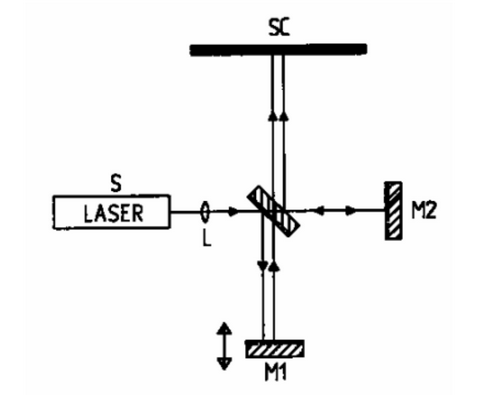
\includegraphics[height=5cm]{imagens/interferometer.png}
\small{\textit{\\Fonte: roteiro experimental.}}
\end{figure}

Como os dois feixes vieram da mesma fonte, as amplitudes e fases iniciais coincidem. Fazendo $I_1 = I_2$ na eq. \eqref{eq: interference formula}, temos
\begin{equation}
\begin{aligned}
\Delta = 2m\pi \implies I(\mathbf{r}) = 4I_1 \;, \\
\Delta = (2m+1)\pi \implies I(\mathbf{r}) = 0 \;.
\end{aligned}
\end{equation}

\noindent A diferença de fase nesse caso será apenas devido ao termo $\mathbf{k} \cdot (\mathbf{r}_2 - \mathbf{r}_1 ) = k_0 n d = 2\pi n d / \lambda_0$, onde $nd$ é a diferença de caminho óptico. 
Devido a periodicidade de $2\pi$ no padrão de interferência, ao contar um número inteiro $m$ de variação de mínimos ou máximos de interferência ao causar uma variação $nd$ no caminho óptico de um caminho em relação ao outro, a seguinte relação será verdadeira:
\begin{equation}
\frac{2\pi n d}{\lambda_0} = 2m\pi \implies \lambda_0 = \frac{nd}{m}.
\end{equation}

